\section{Turret Design}
\label{turretdesign}
As mentioned in the section on requirements, the turret needs to be able to detect, aim and fire at a moving target. 
From a design perspective two distinct properties namely, horizontal and vertical rotation are needed. There are of course many different ways of achieving both, but in this case the simplest thing would be to have one servo motor handle vertical rotation and another servo motor handle horizontal rotation. 

The group started with the model depicted in \autoref{first_model}.

\begin{figure}[hptb]
  \centering
    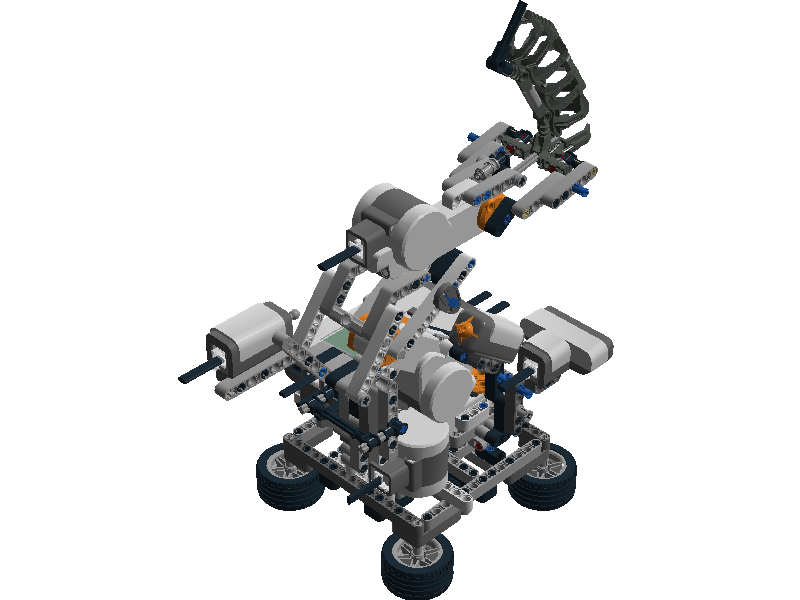
\includegraphics[width=0.5\textwidth]{img/Step114.png}
  \caption{Initial model for the projectile launcher}
  \label{first_model}
\end{figure}

However the construction was too top heavy thus making it difficult to achieve a precise and reliable rotation. Attempts were made, but the group was unable to find an acceptable solution. The main problem was that a single servo was responsible for rotating the everything except the base, and the servo even had to handle its own weight. 

\autoref{final_model} shows the final design of the turret. The focus was on a relatively compact design, minimizing the weight on the rotating platform. The vertical raising mechanism was refactored to a minimal set of components and the horizontal rotation was redesigned in such a way that the servo could be moved from the tower to the base. 

The rotation was restricted to a fixed set of degrees. This decision was based on the hardware analysis where it was discovered that the Kinect's field of view covers 57 horizontal degrees and 34 vertical degrees. 

The altered design meant that the NXT and the Kinect did not have to be placed on the turret, but rather behind and in front of the turret. The servo that handles horizontal rotation was placed on a structure next to the turret. And lastly there was need for some way of configuring the starting position of the turret, in order to be absolutely sure that the turret was facing in the same direction on every initialization. A touch sensor was placed next to the turret and a beam was mounted onto the turret that would hit the sensor at a certain angle. It should also be noted that the competition cannon in \autoref{competition_cannon} is not included in LEGO Digital Designer, which was used to make the model, and therefore the cannon is missing from the model in \autoref{final_model}.

\begin{figure}[hptb]
  \centering
    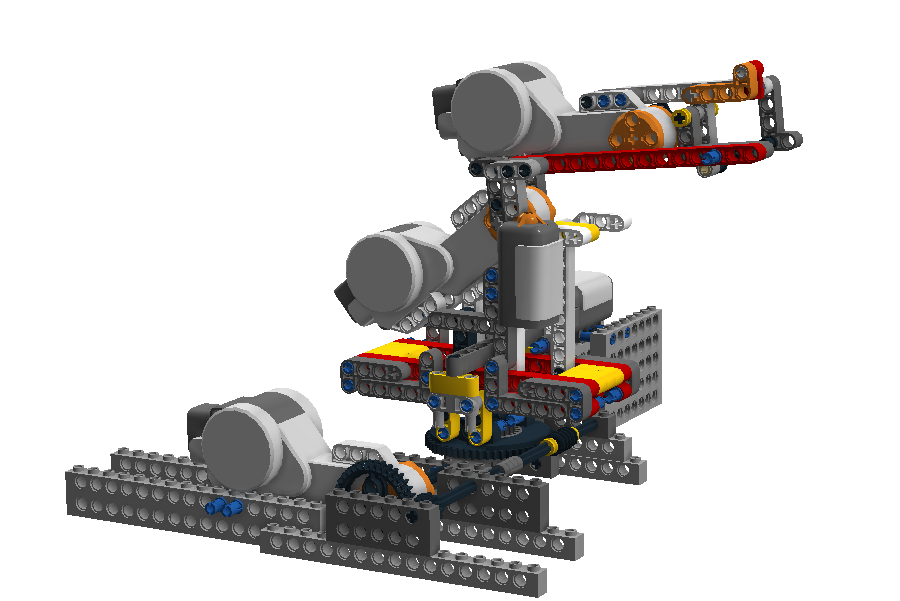
\includegraphics[width=0.5\textwidth]{img/design_turret4.png}
  \caption{Final model of the projectile launcher.}
  \label{final_model}
\end{figure}

\subsection{Placing the Kinect} % (fold)
\label{sub:placing_the_kinect}
There are several options with regards to the placement of the Kinect in relation to the turret. 

An approach would be to place the Kinect behind or next to the turret, with the turret within the Kinect's field of vision. This would enable the Kinect to calculate the target's position and speed in relation to the turret. The problem is that the turret would also obstruct the Kinect's field of vision, resulting in irregularities and might even lead to false results.

A third approach, and the one chosen for implementation, is to place the Kinect right in front of the turret, directly under the cannon. In this case the NXT only has to factor in the height difference between the Kinect and the cannon. The Kinect can only see a limited amount of degrees on the horizontal axis, and the turret is designed to be able to rotate accordingly. Thus fulfilling the requirements.
%subsection placing_the_kinect (end)